\documentclass[11pt]{beamer}
\usepackage[utf8]{inputenc}
\usepackage[T1]{fontenc}
\usepackage{lmodern}
\usepackage{amsmath}
\usepackage{amsfonts}
\usepackage{amssymb}
\usepackage{graphicx}
\usetheme{Luebeck}
\usecolortheme{albatross}
\begin{document}
	\author{Anthony Odenthal - KE7OSN}
	\title{An Introduction to Event Support}
	\subtitle{A practical guide to helpping out}
	%\logo{}
	%\institute{}
	\date{16 September 2019}
	%\subject{}
	%\setbeamercovered{transparent}
	%\setbeamertemplate{navigation symbols}{}
\AtBeginSection[]
{
	\begin{frame}
	\frametitle{Table of Contents}
	\tableofcontents[currentsection]
	\end{frame}
}

\begin{frame}[plain]
	\maketitle
\end{frame}

\begin{frame}{Table of Contents}
\tableofcontents
\end{frame}

\section{Introduction}

\begin{frame}
\frametitle{Preface}
Supporting community events can be a lot of fun, and great practice for emergencies.
\end{frame}

\begin{frame}{Little bit of legwork}
Poor planning and execution can cause loads of headaches and leave a bad taste for everyone.
\end{frame}

\subsection{Practice}

\begin{frame}{Practice}
The basic principles of event support are the same as disaster support.
\end{frame}

\begin{frame}{Pass the message}
Every event will have some information that needs to get moved from one location to another (or several others). Being able to quickly and accurately pass the important information helps everyone do their job. And can be very important for keeping everyone safe.
\end{frame}

\begin{frame}
	\begin{center}
		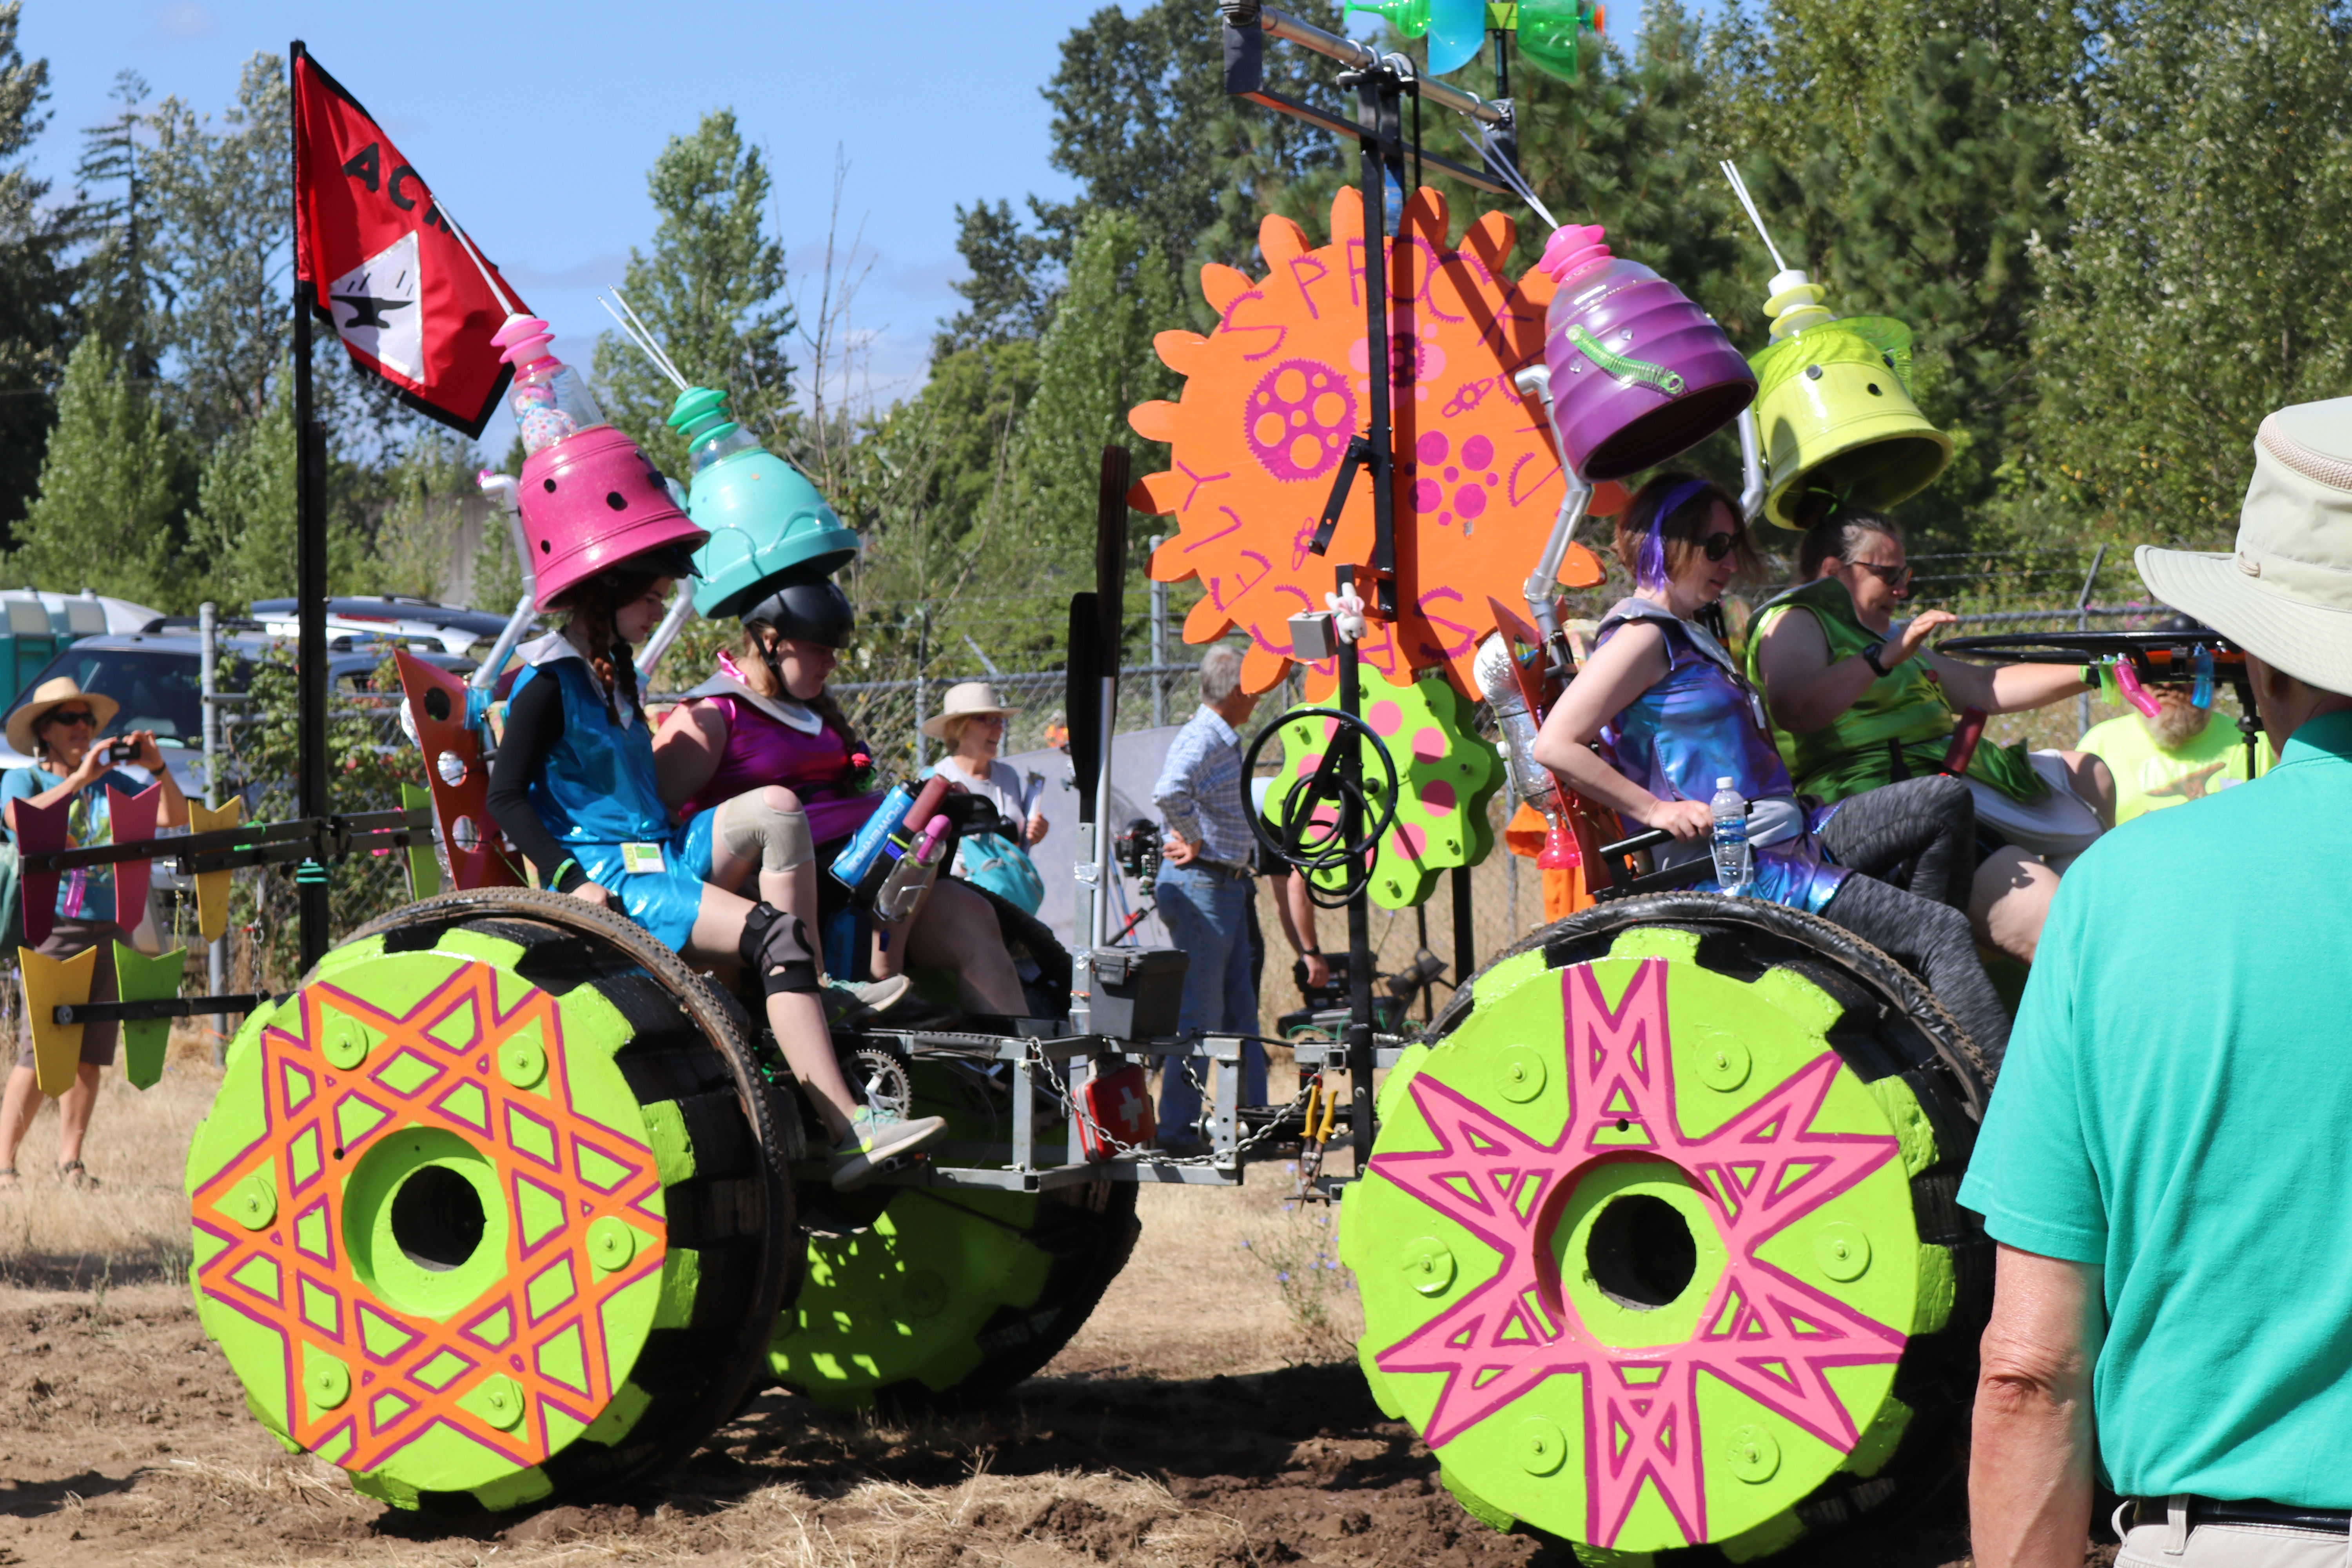
\includegraphics[height=.8\textheight]{media/IMG_1055.JPG}
	\end{center}

\end{frame}

\subsection{Equipment}

\begin{frame}
	Events are also a good chance to try and shakedown equipment. New radio, old radio, different antenna setup.
	See how everything works in the real world
\end{frame}

\subsection{Fun!}

\begin{frame}
	Also these things are a lot of FUN!
\end{frame}

\begin{frame}
	\begin{center}
		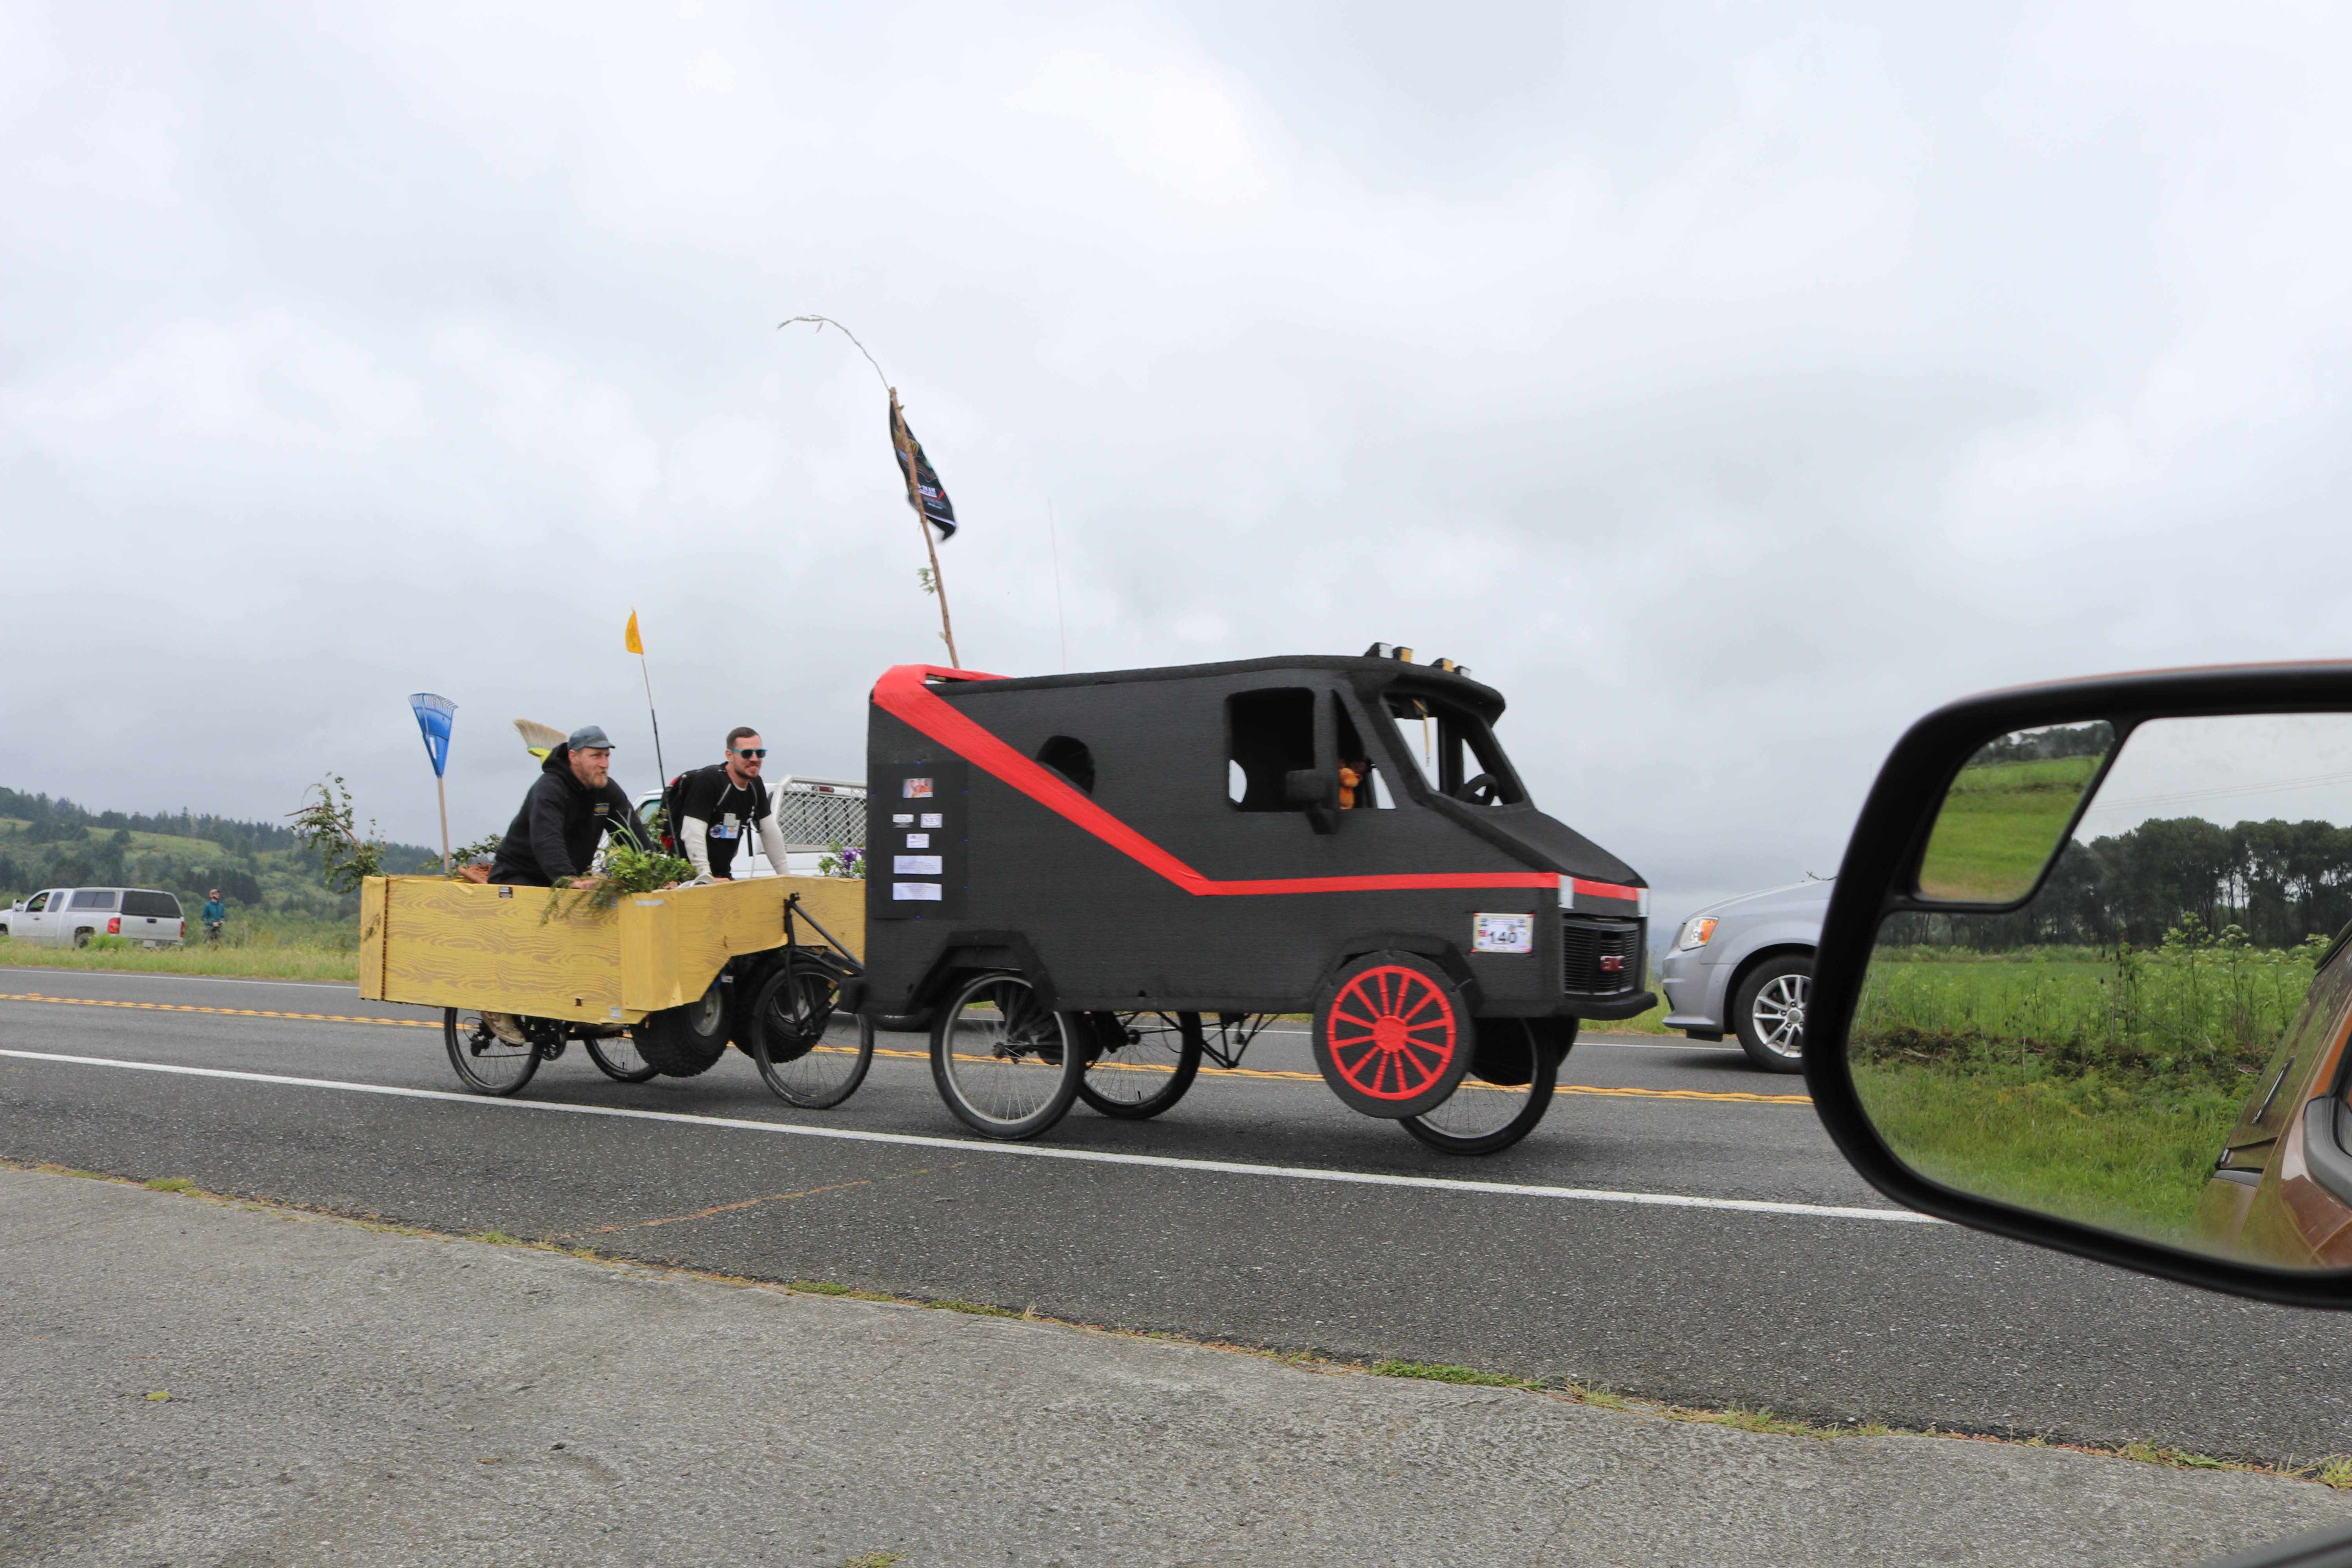
\includegraphics[height=.8\textheight]{media/IMG_3272.JPG}
	\end{center}
\end{frame}
\section{Planning}

\begin{frame}
	Every good event starts with a good plan. You must determine a few things as early as possible.
	\begin{itemize}
		\item What are you there to do?
		\item When and Where?
		\item Is ham radio a good fit?
		\item How many people?
		\item Do you have the coverage you need?
	\end{itemize}
\end{frame}

\subsection{What to do}
\begin{frame}
	One of the first things is to find out what they need you to do? Are you keeping track of people, timing, just there to pass messages, or all of the above. Figuring out what the workload looks like will help you decide how many people you need and if you can handle everything.
\end{frame}

\subsection{Who, what, when, why, where, how?}
\begin{frame}
	When and where, sounds obvious but for more than just telling people where to go. Finding out repeater/simplex coverage antenna locations, etc. Also knowing if there are other weather related precautions volunteers need to make
\end{frame}

\begin{frame}
	\begin{center}
	\includegraphics[height=.8\textheight]{media/Annotation-2019-09-14-084812.png}
	\end{center}
\end{frame}

\begin{frame}
	How many people do you need? You need to be upfront and realistic about the number of people you can provide, and how much they can do. Volunteers have other things to do, and the sooner you can ask for help the better. It is also important to let people know if they need to be mobile.
\end{frame}

\subsection{Good fit?}
\begin{frame}
	Early on determine if the event is a good fit for ham radio. Some event organizers are really just looking for radios for their people. For some events the traffic isn't a good fit with ham radio. We can still help advise event coordinators, but may not be useful day-of.
\end{frame}

\begin{frame}
	Are you going to be using HF, repeaters, simplex? Can you communicate with all the locations you need to? Do you need people with special equipment or abilities at specific locations?
\end{frame}

\begin{frame}
	\begin{center}
		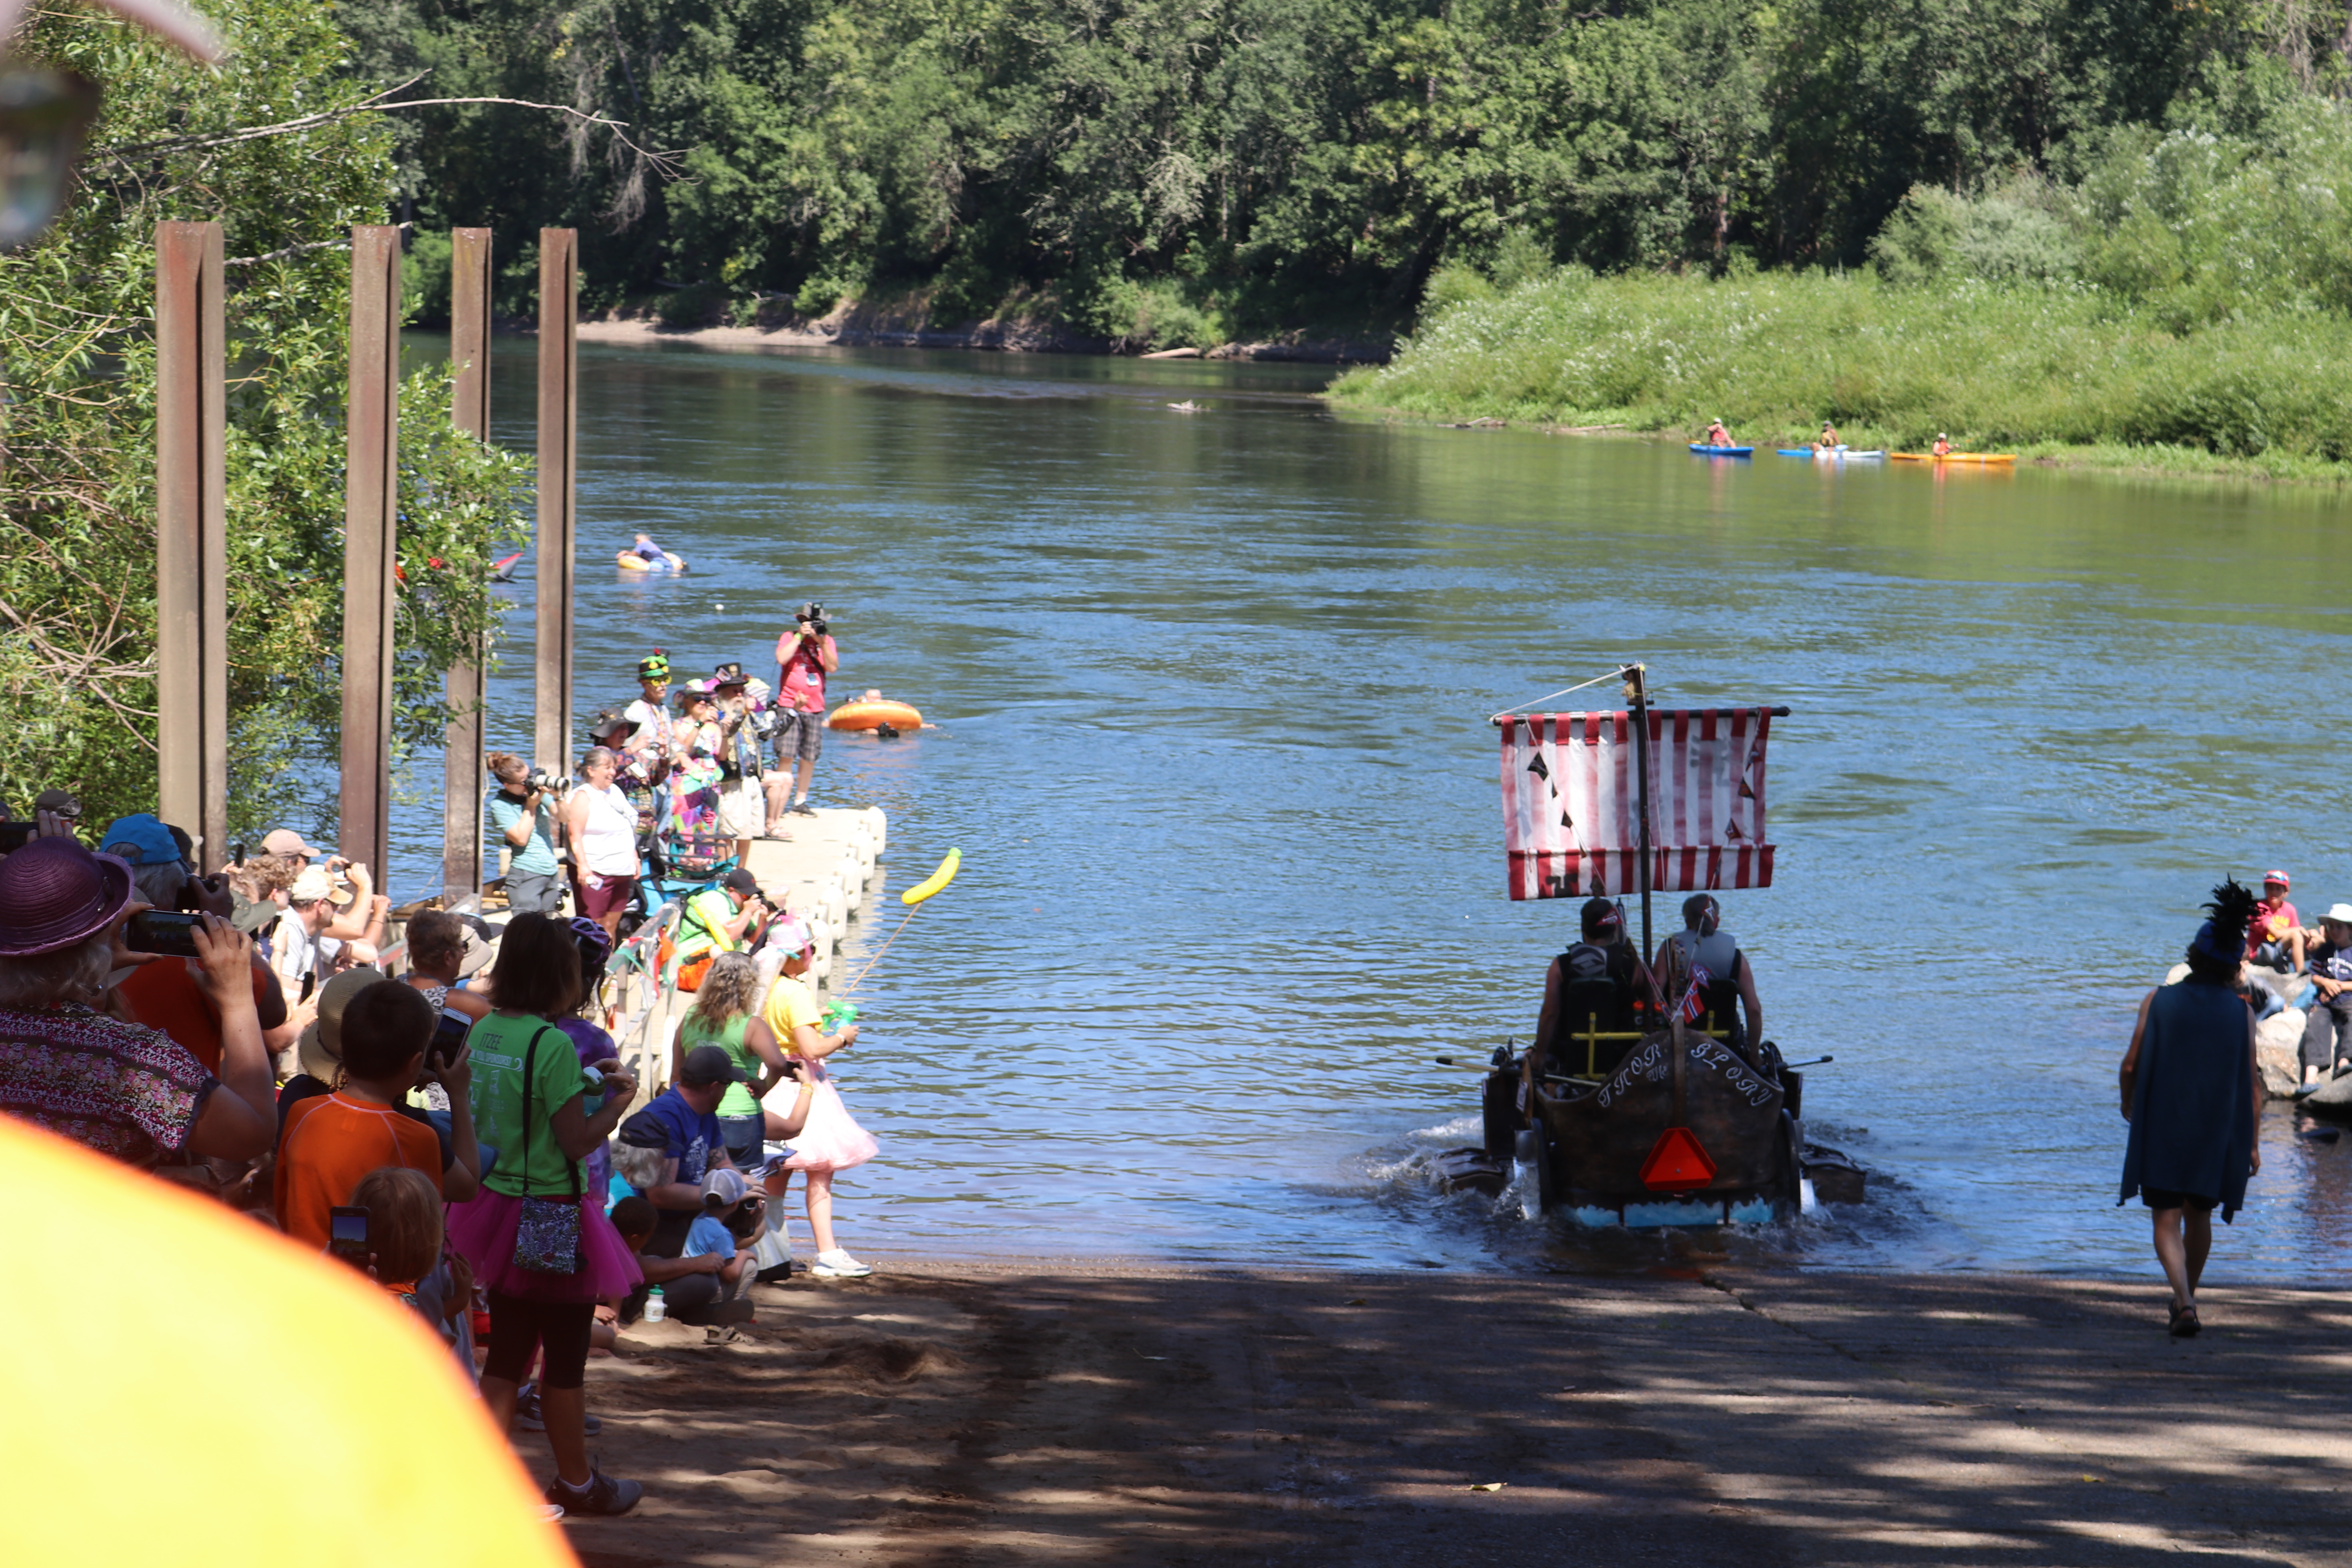
\includegraphics[height=.8\textheight]{media/IMG-2019-07-21-11513547.JPG}
	\end{center}
\end{frame}

\begin{frame}
	Determine contingency, and emergency plans. What happens if someone gets hurt? Who do you call if supplies run low? Backup frequencies?
\end{frame}

\begin{frame}
	It is often helpful to prepare packets of information to hand out to volunteers. Have the plan, emergency contacts, frequencies, and other useful information.
	Bonus points if you print it out on waterproof paper for those wet locations.
\end{frame}

\begin{frame}
	Recruit your volunteers!
	Make sure you communicate specific requirements, and benefits.
\end{frame}

\begin{frame}
	Point out specific hazards
\end{frame}

\subsection{Pictures}

\begin{frame}
	\begin{center}
		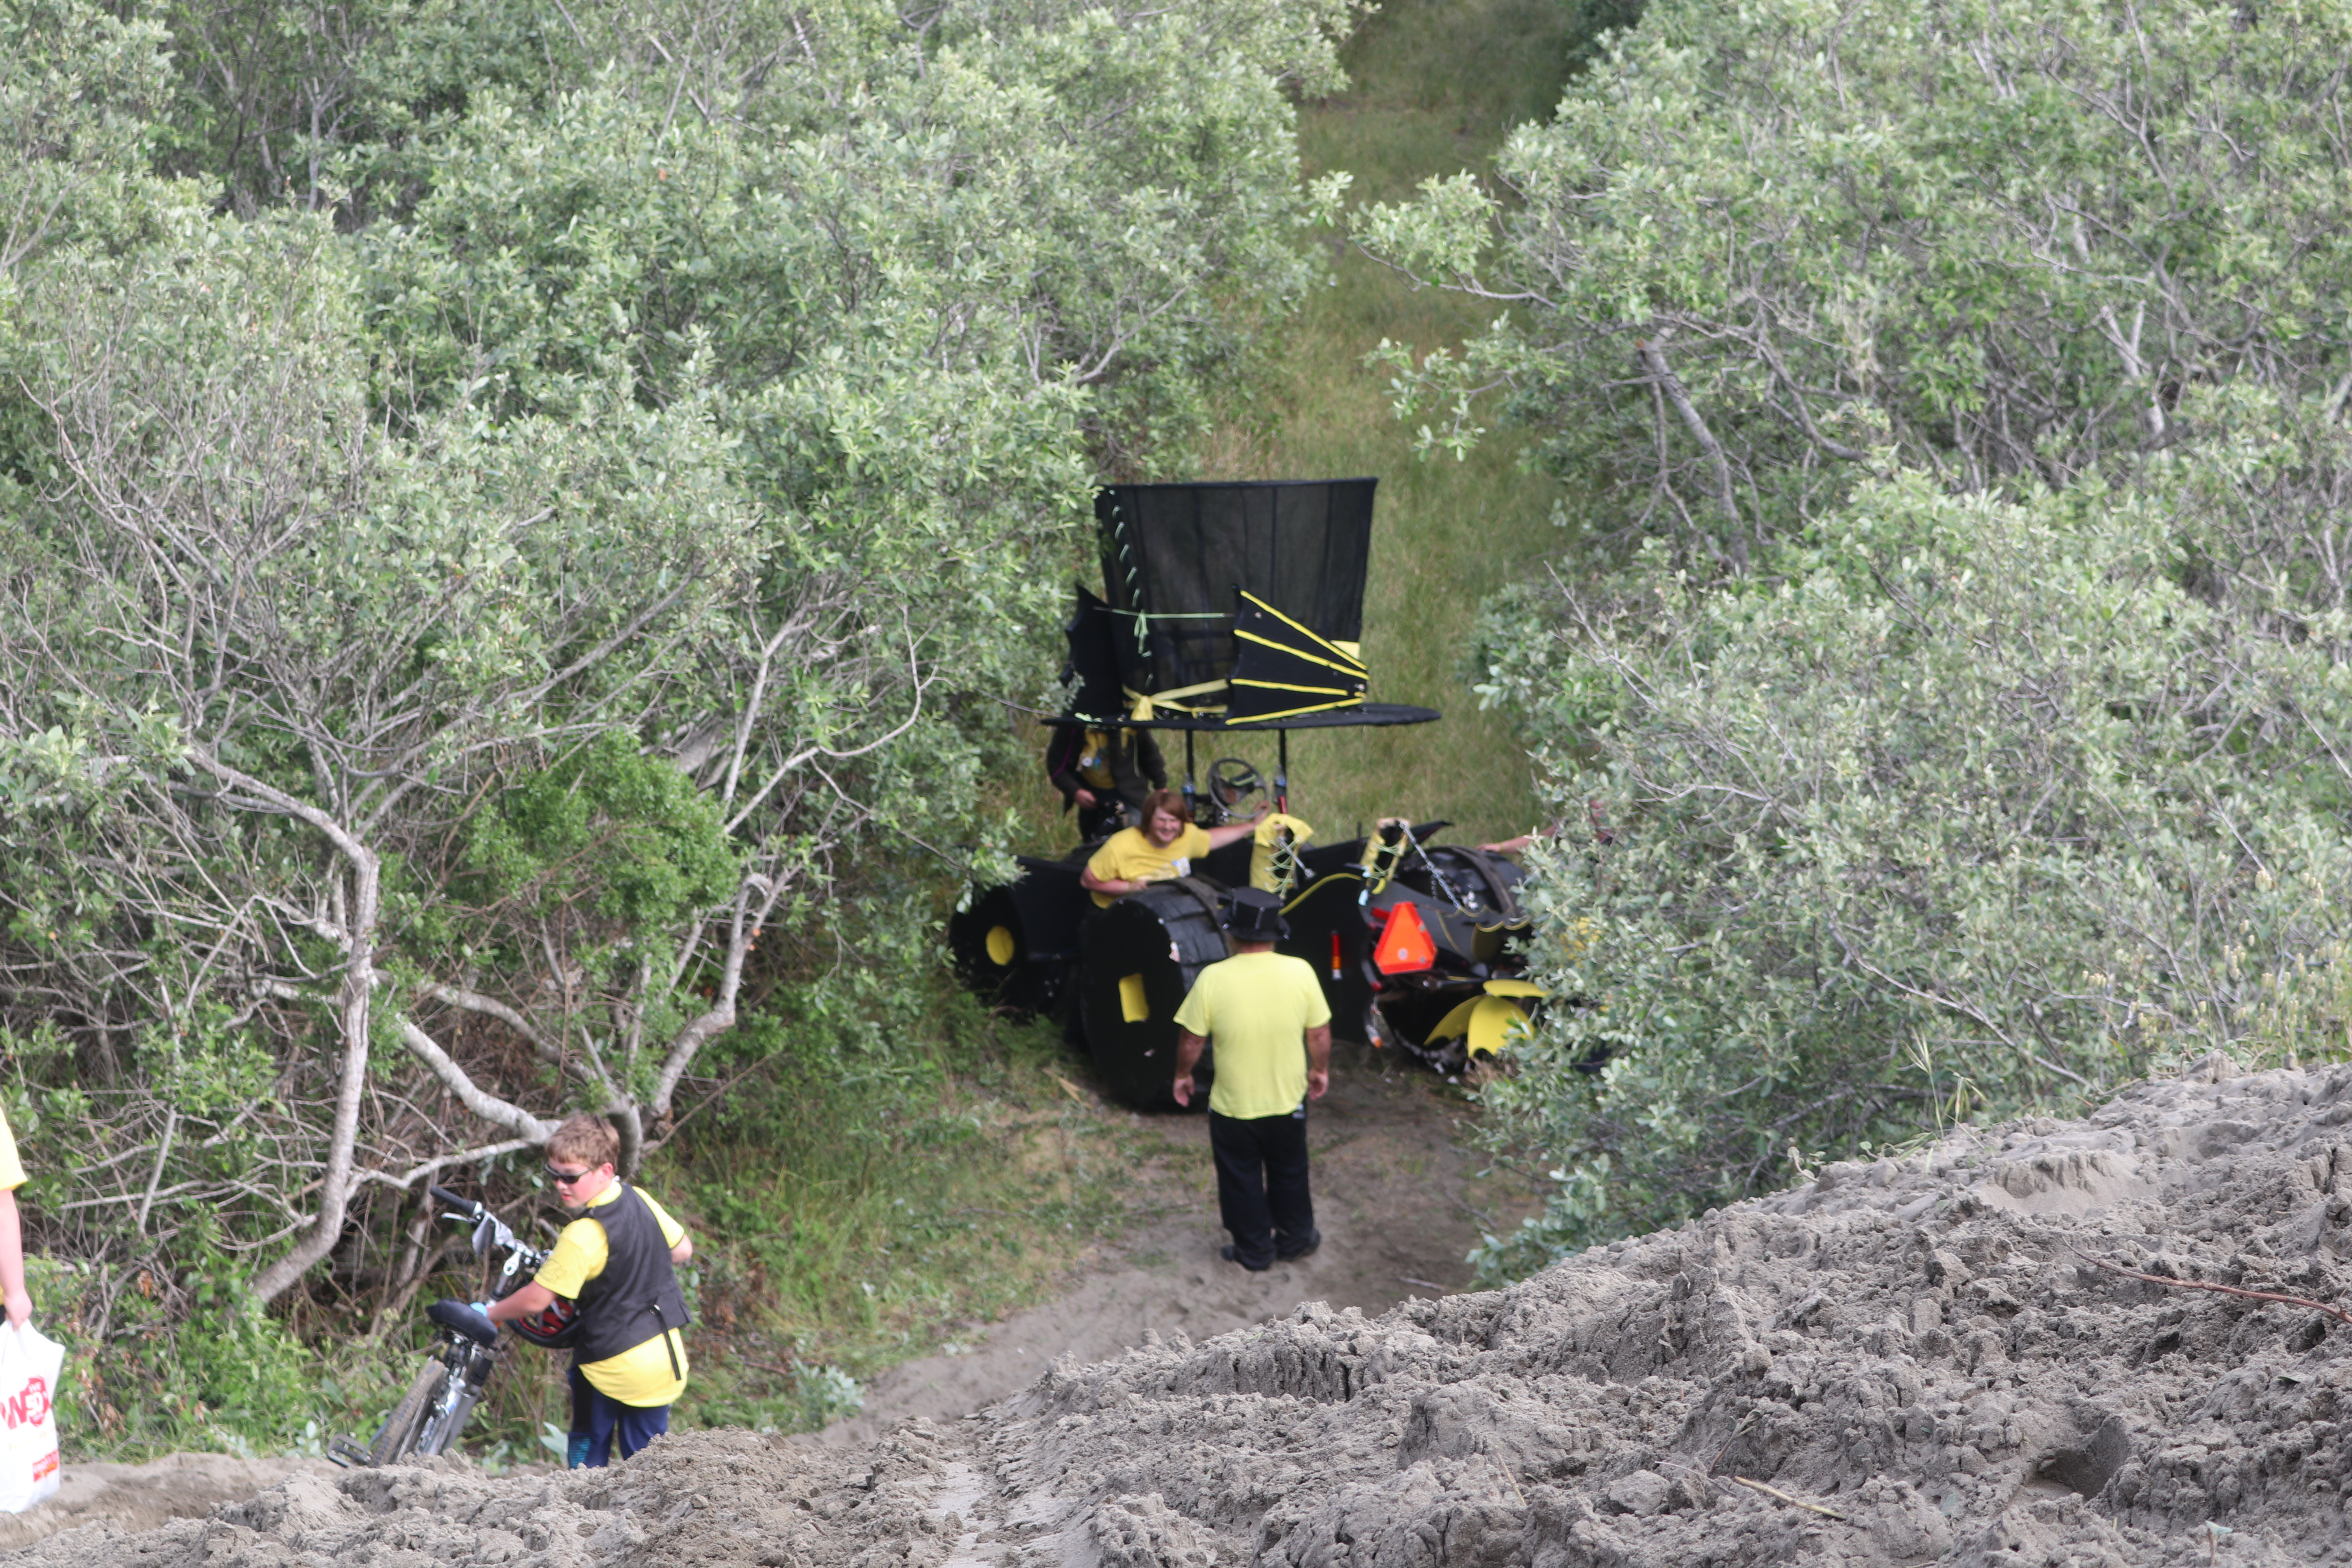
\includegraphics[height=.8\textheight]{media/IMG_2145.JPG}
	\end{center}
\end{frame}

\begin{frame}
	\begin{center}
		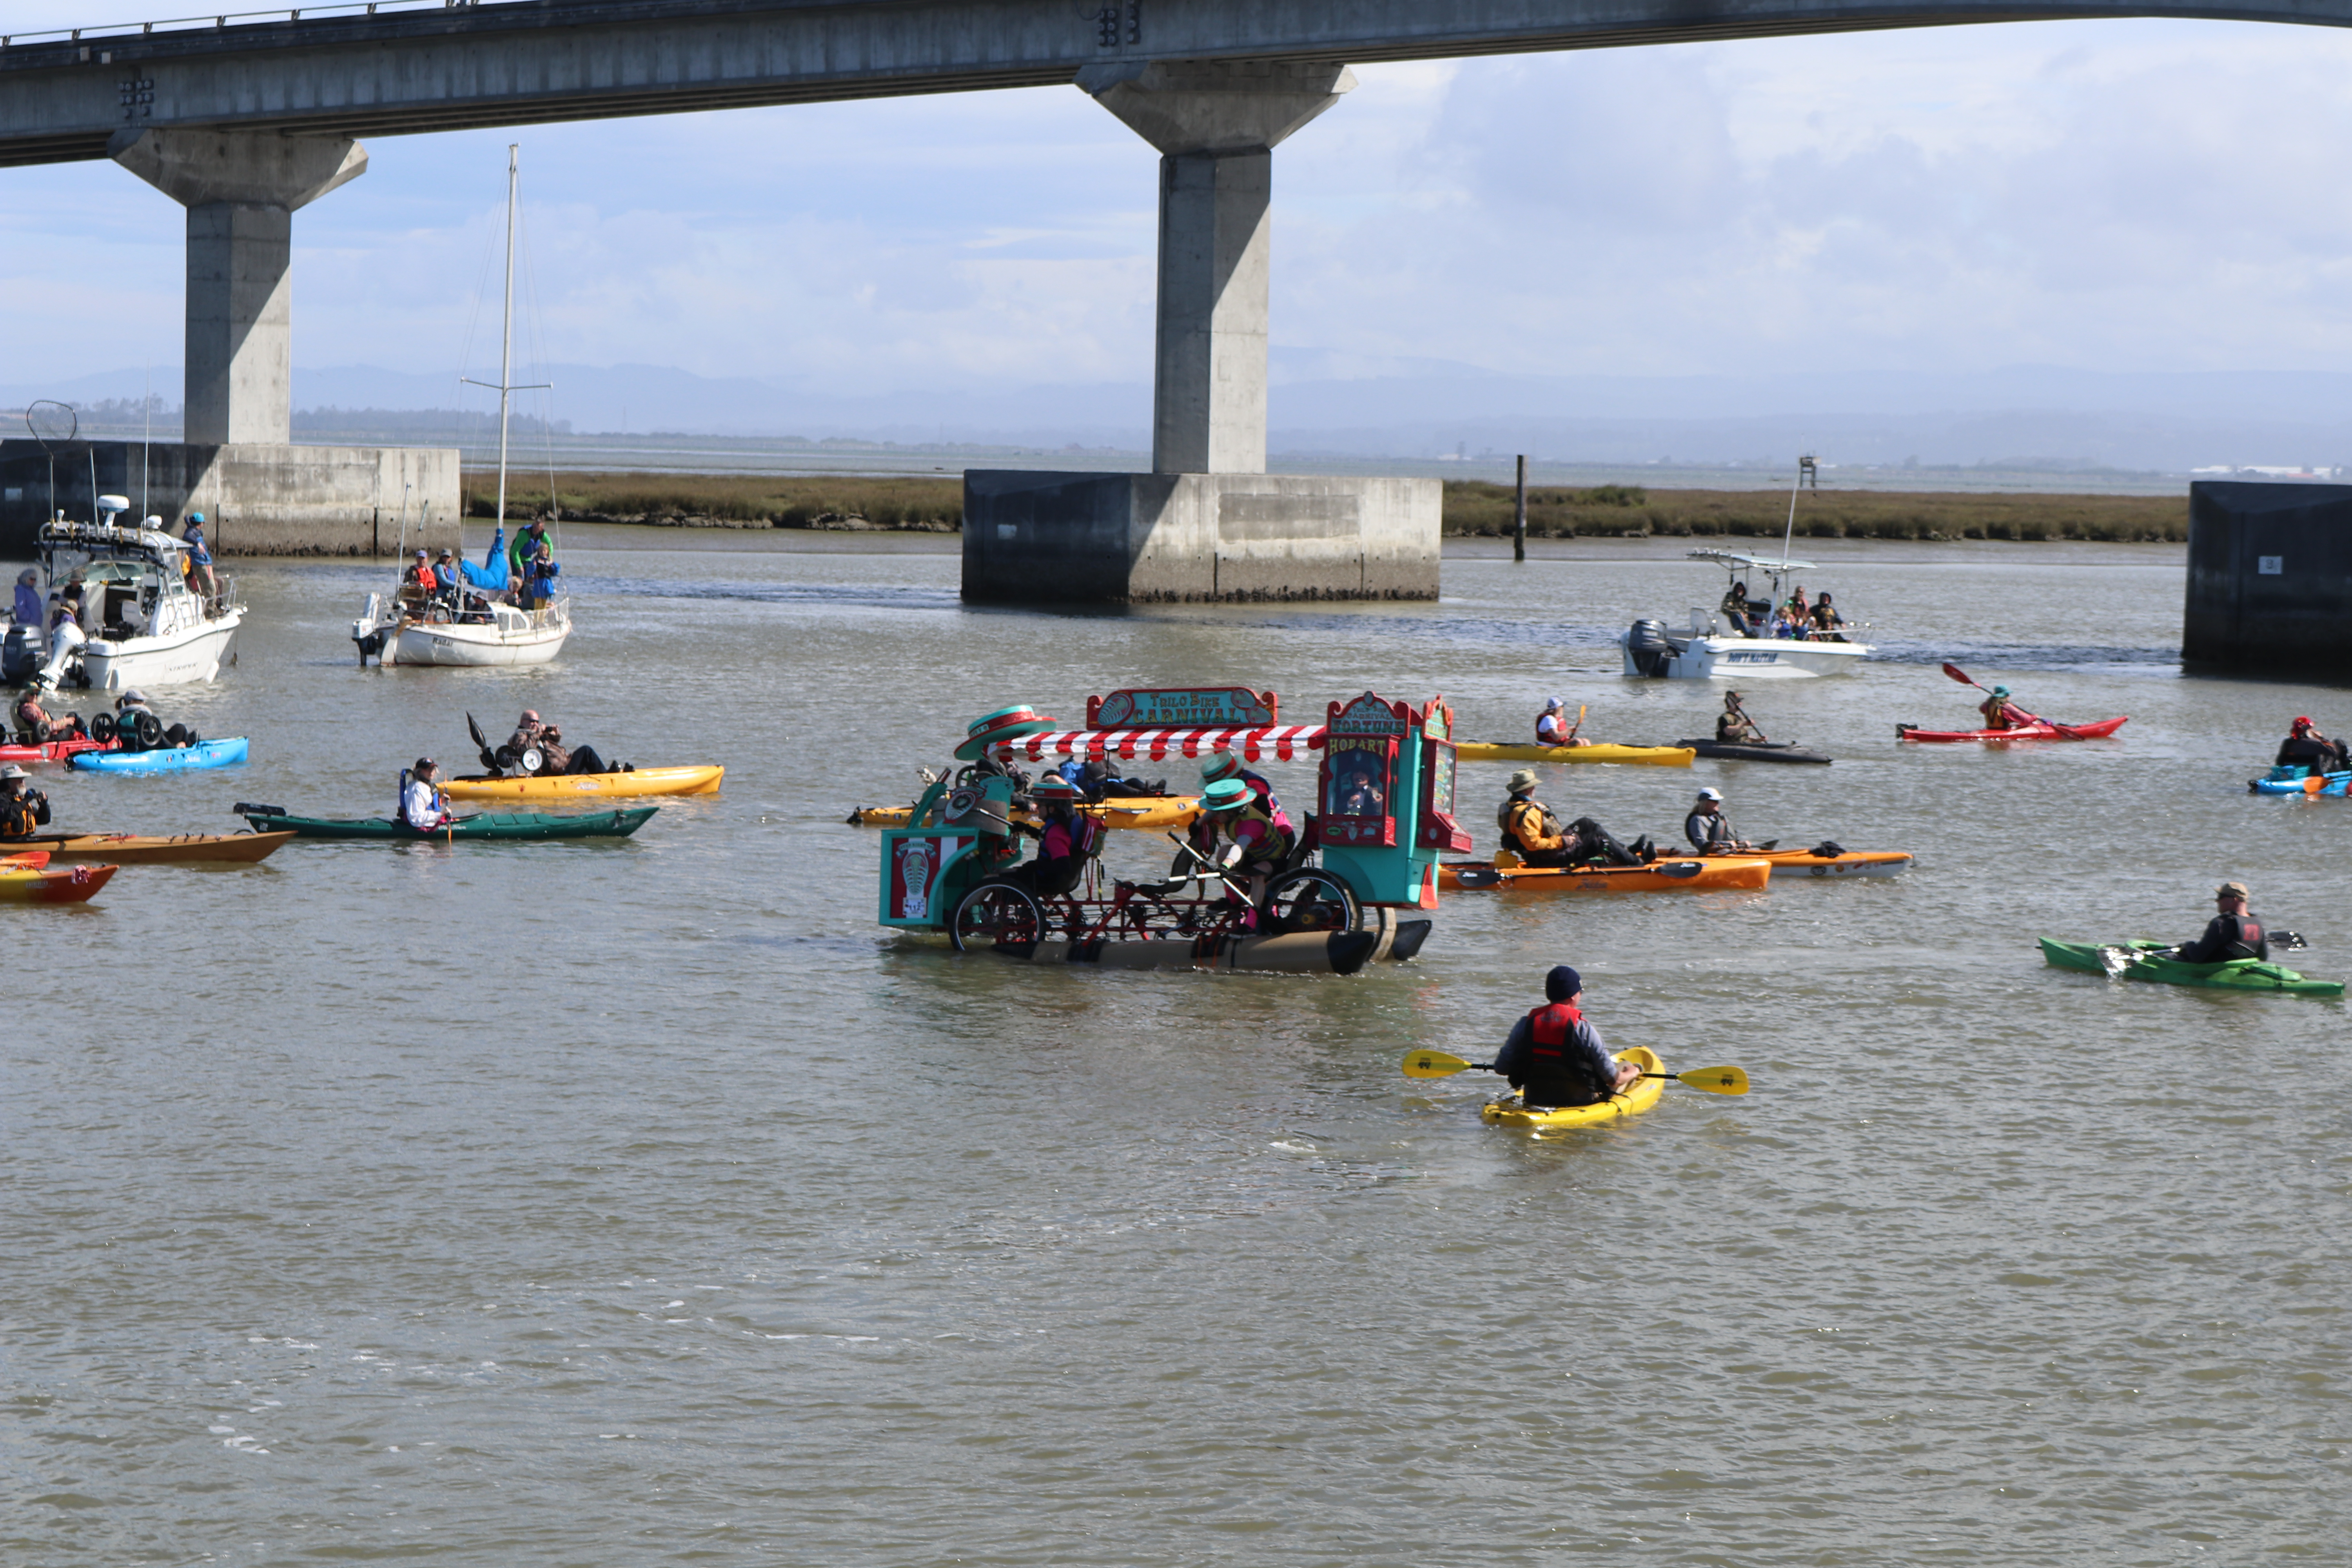
\includegraphics[height=.8\textheight]{media/IMG_2988.JPG}
	\end{center}
\end{frame}

\begin{frame}
	\begin{center}
		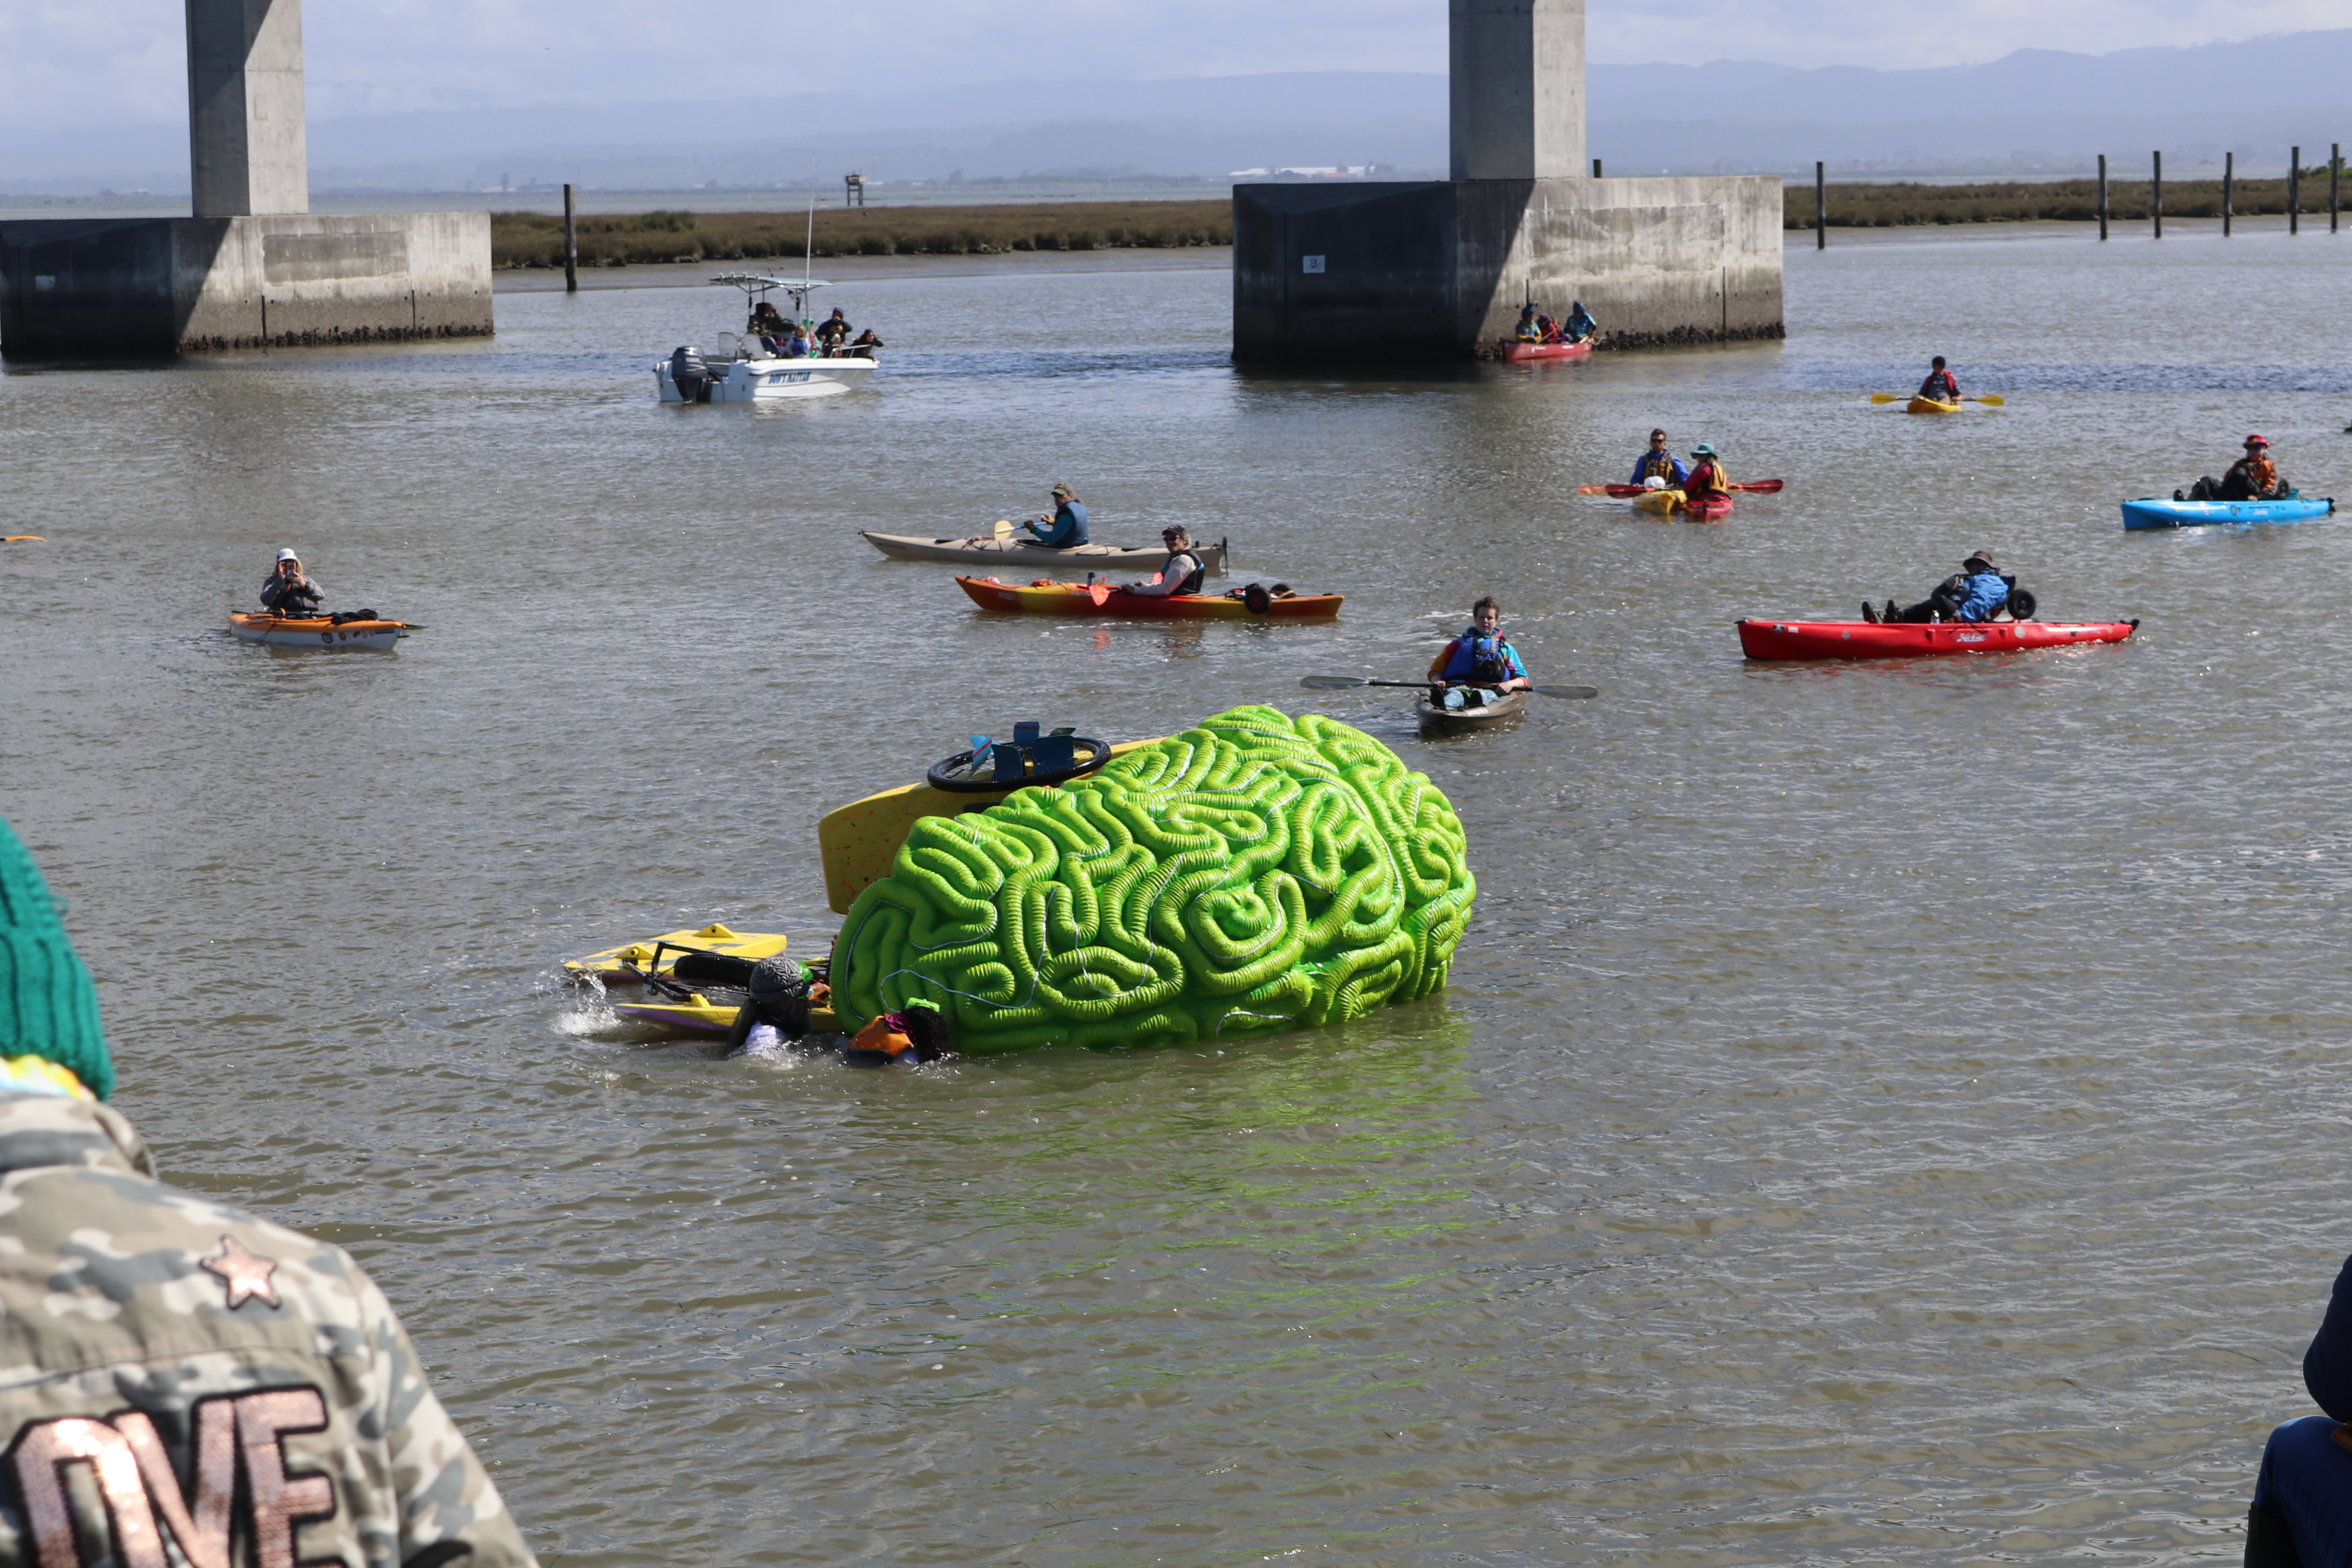
\includegraphics[height=.8\textheight]{media/IMG_2992.JPG}
	\end{center}
\end{frame}

\begin{frame}
	Be sure to keep in communication with the stakeholders. You win a lot of brownie points for having information ready before they ask.
\end{frame}

\begin{frame}
	Be flexible, things will change. Be ready to roll with it.
\end{frame}

\section{Volunteering}

\subsection{Communicate}

\begin{frame}
	Save the date. Last minute things come up, but the volunteers are rarely overabundant. Especially radio operators
\end{frame}

\begin{frame}
	Know you limits. Some postings may require standing for long periods, or packing gear in off the road. The more the organizer knows the better they can find the best fit for everyone.
\end{frame}

\begin{frame}
	Changes come up. Just make sure to communicate when they do. If you move, or are going to try something different let someone know.
\end{frame}

\subsection{The Plan, The Goal, The Objectives}

\begin{frame}
	Understand what the goals are, and keep as close to the plan as possible and still get the job done. Going off script may cause more harm than good.
\end{frame}

\begin{frame}
	Be ready and able to help. A little enthusiasm can go a long way too. Especially for fun events, the more you get into it, the more you will get out of it.
\end{frame}

\begin{frame}
	Show up early, and test your gear. It is really important that you know what does and doesn't work in case something goes wrong.
\end{frame}

\subsection{Have FUN!}

\begin{frame}
	Have Fun!
\end{frame}

\begin{frame}
	\begin{center}
		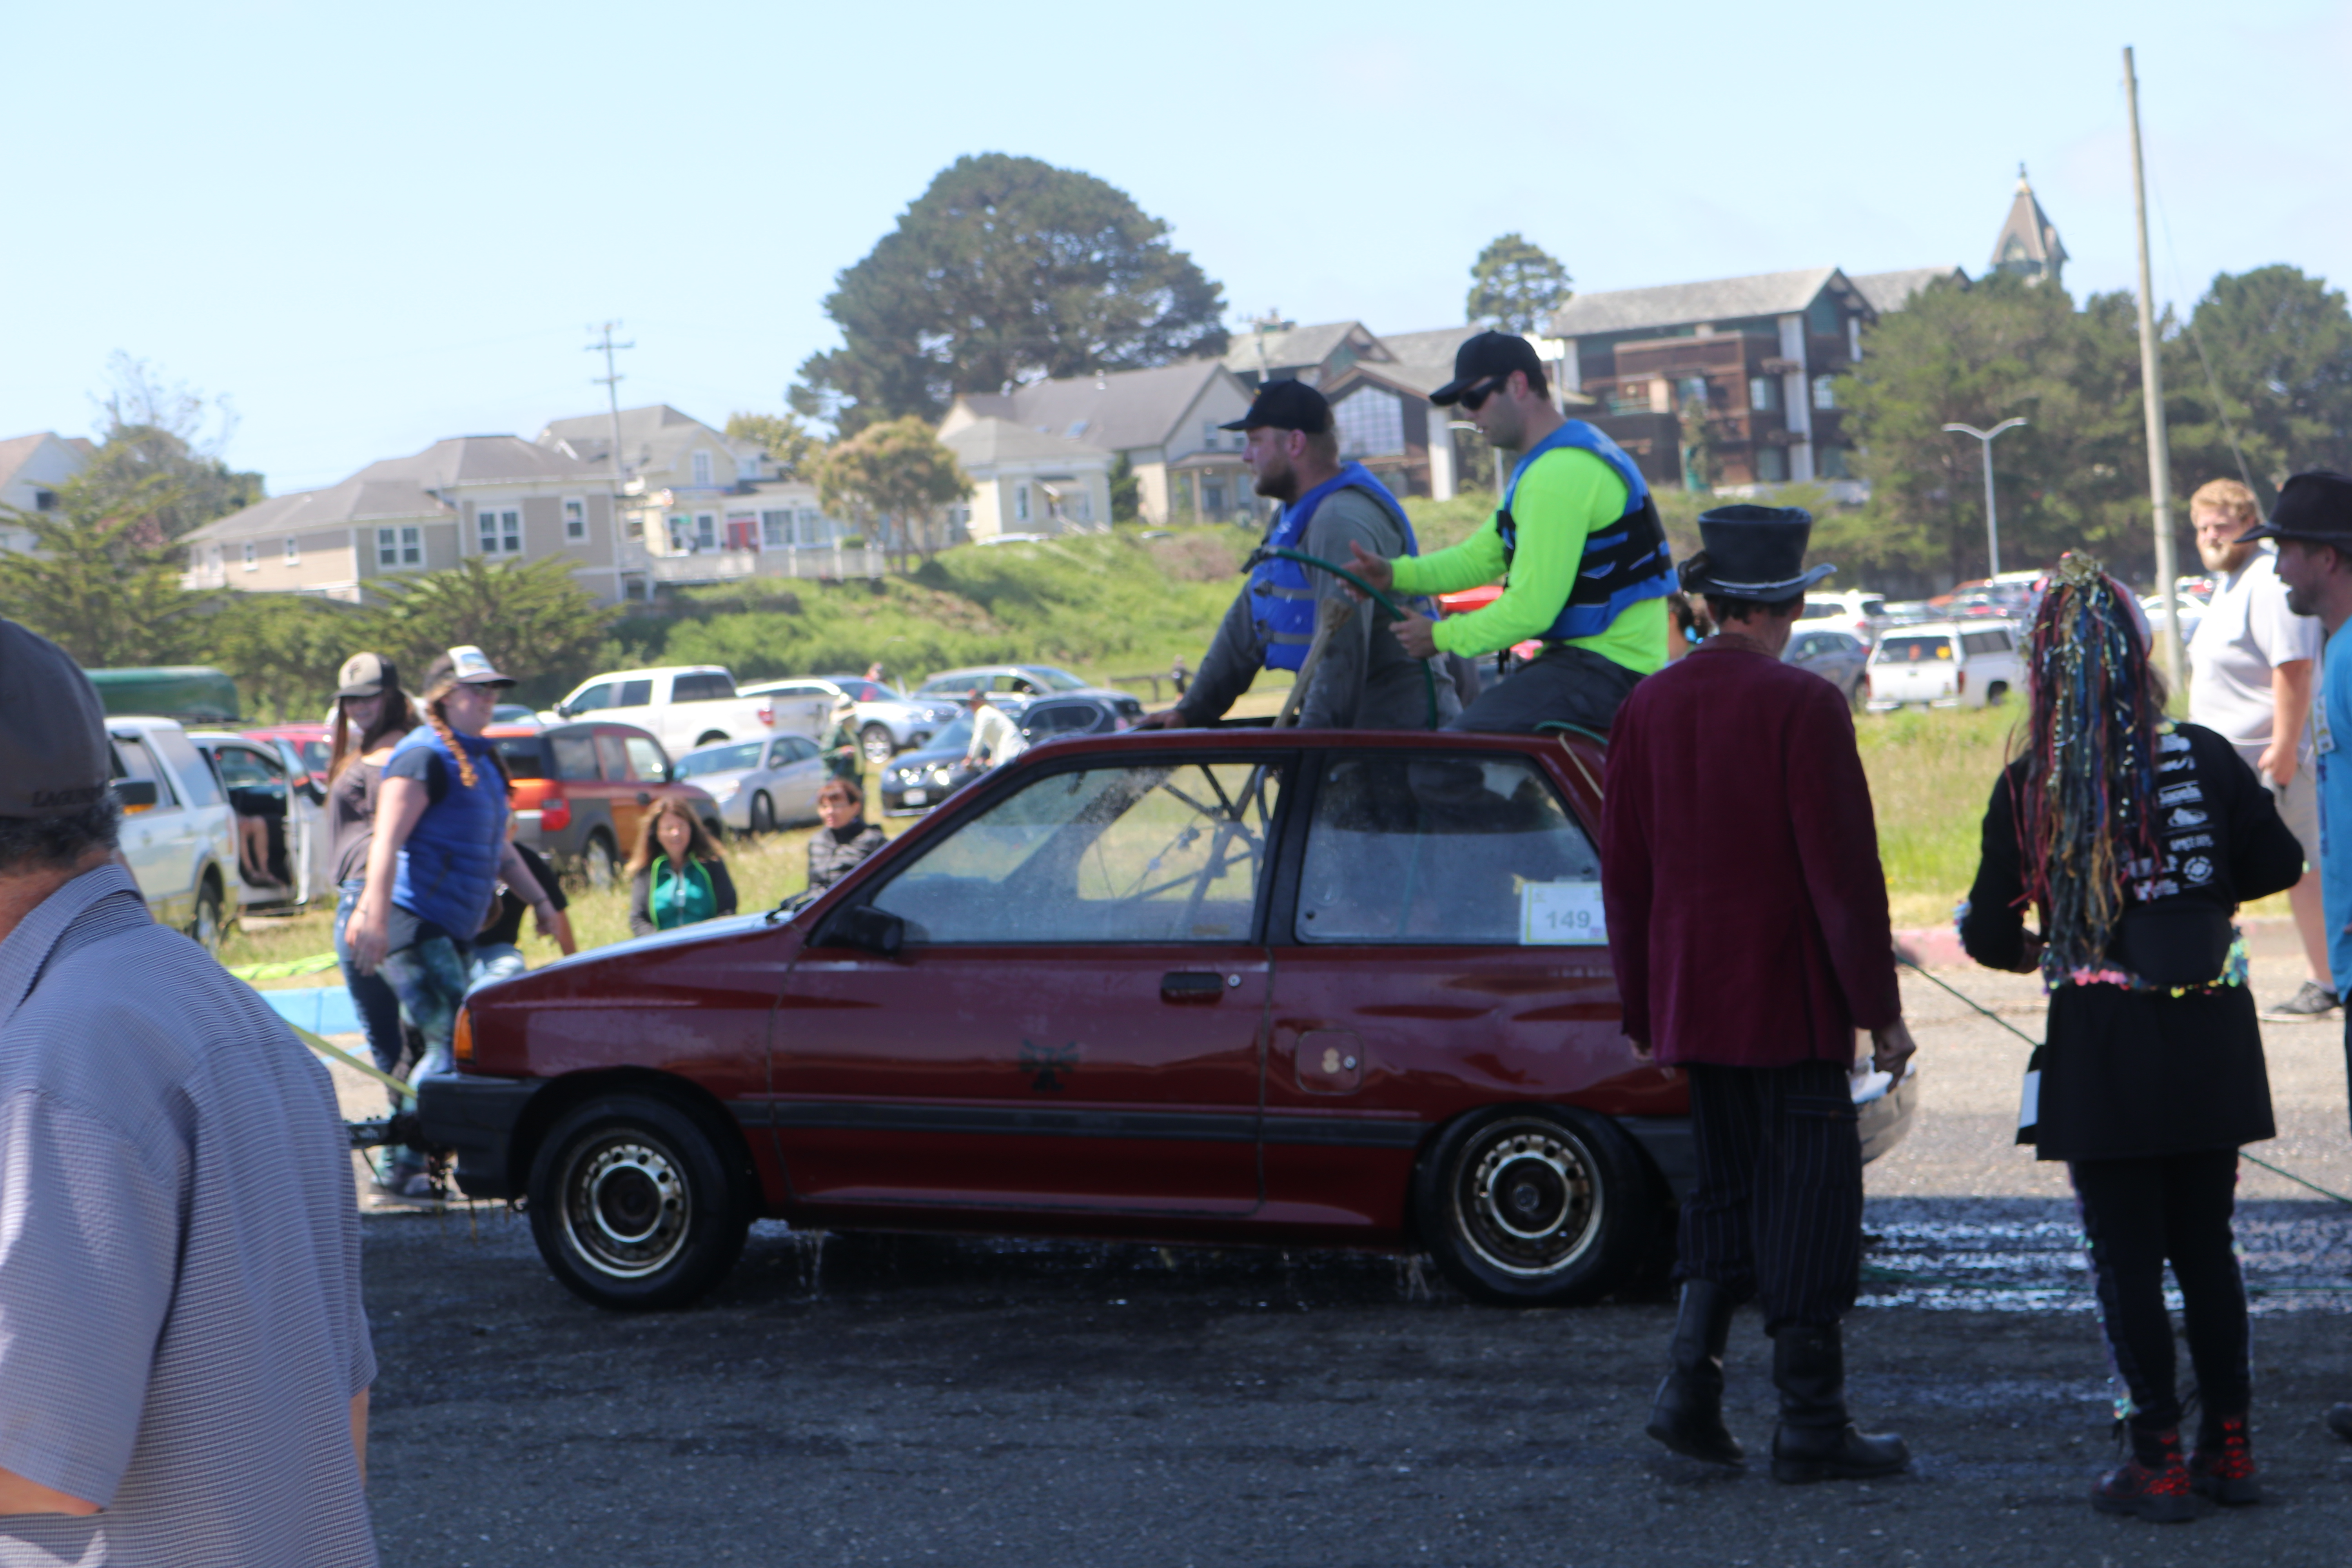
\includegraphics[height=.8\textheight]{media/IMG_2254.JPG}
	\end{center}
\end{frame}

\begin{frame}
	\begin{center}
		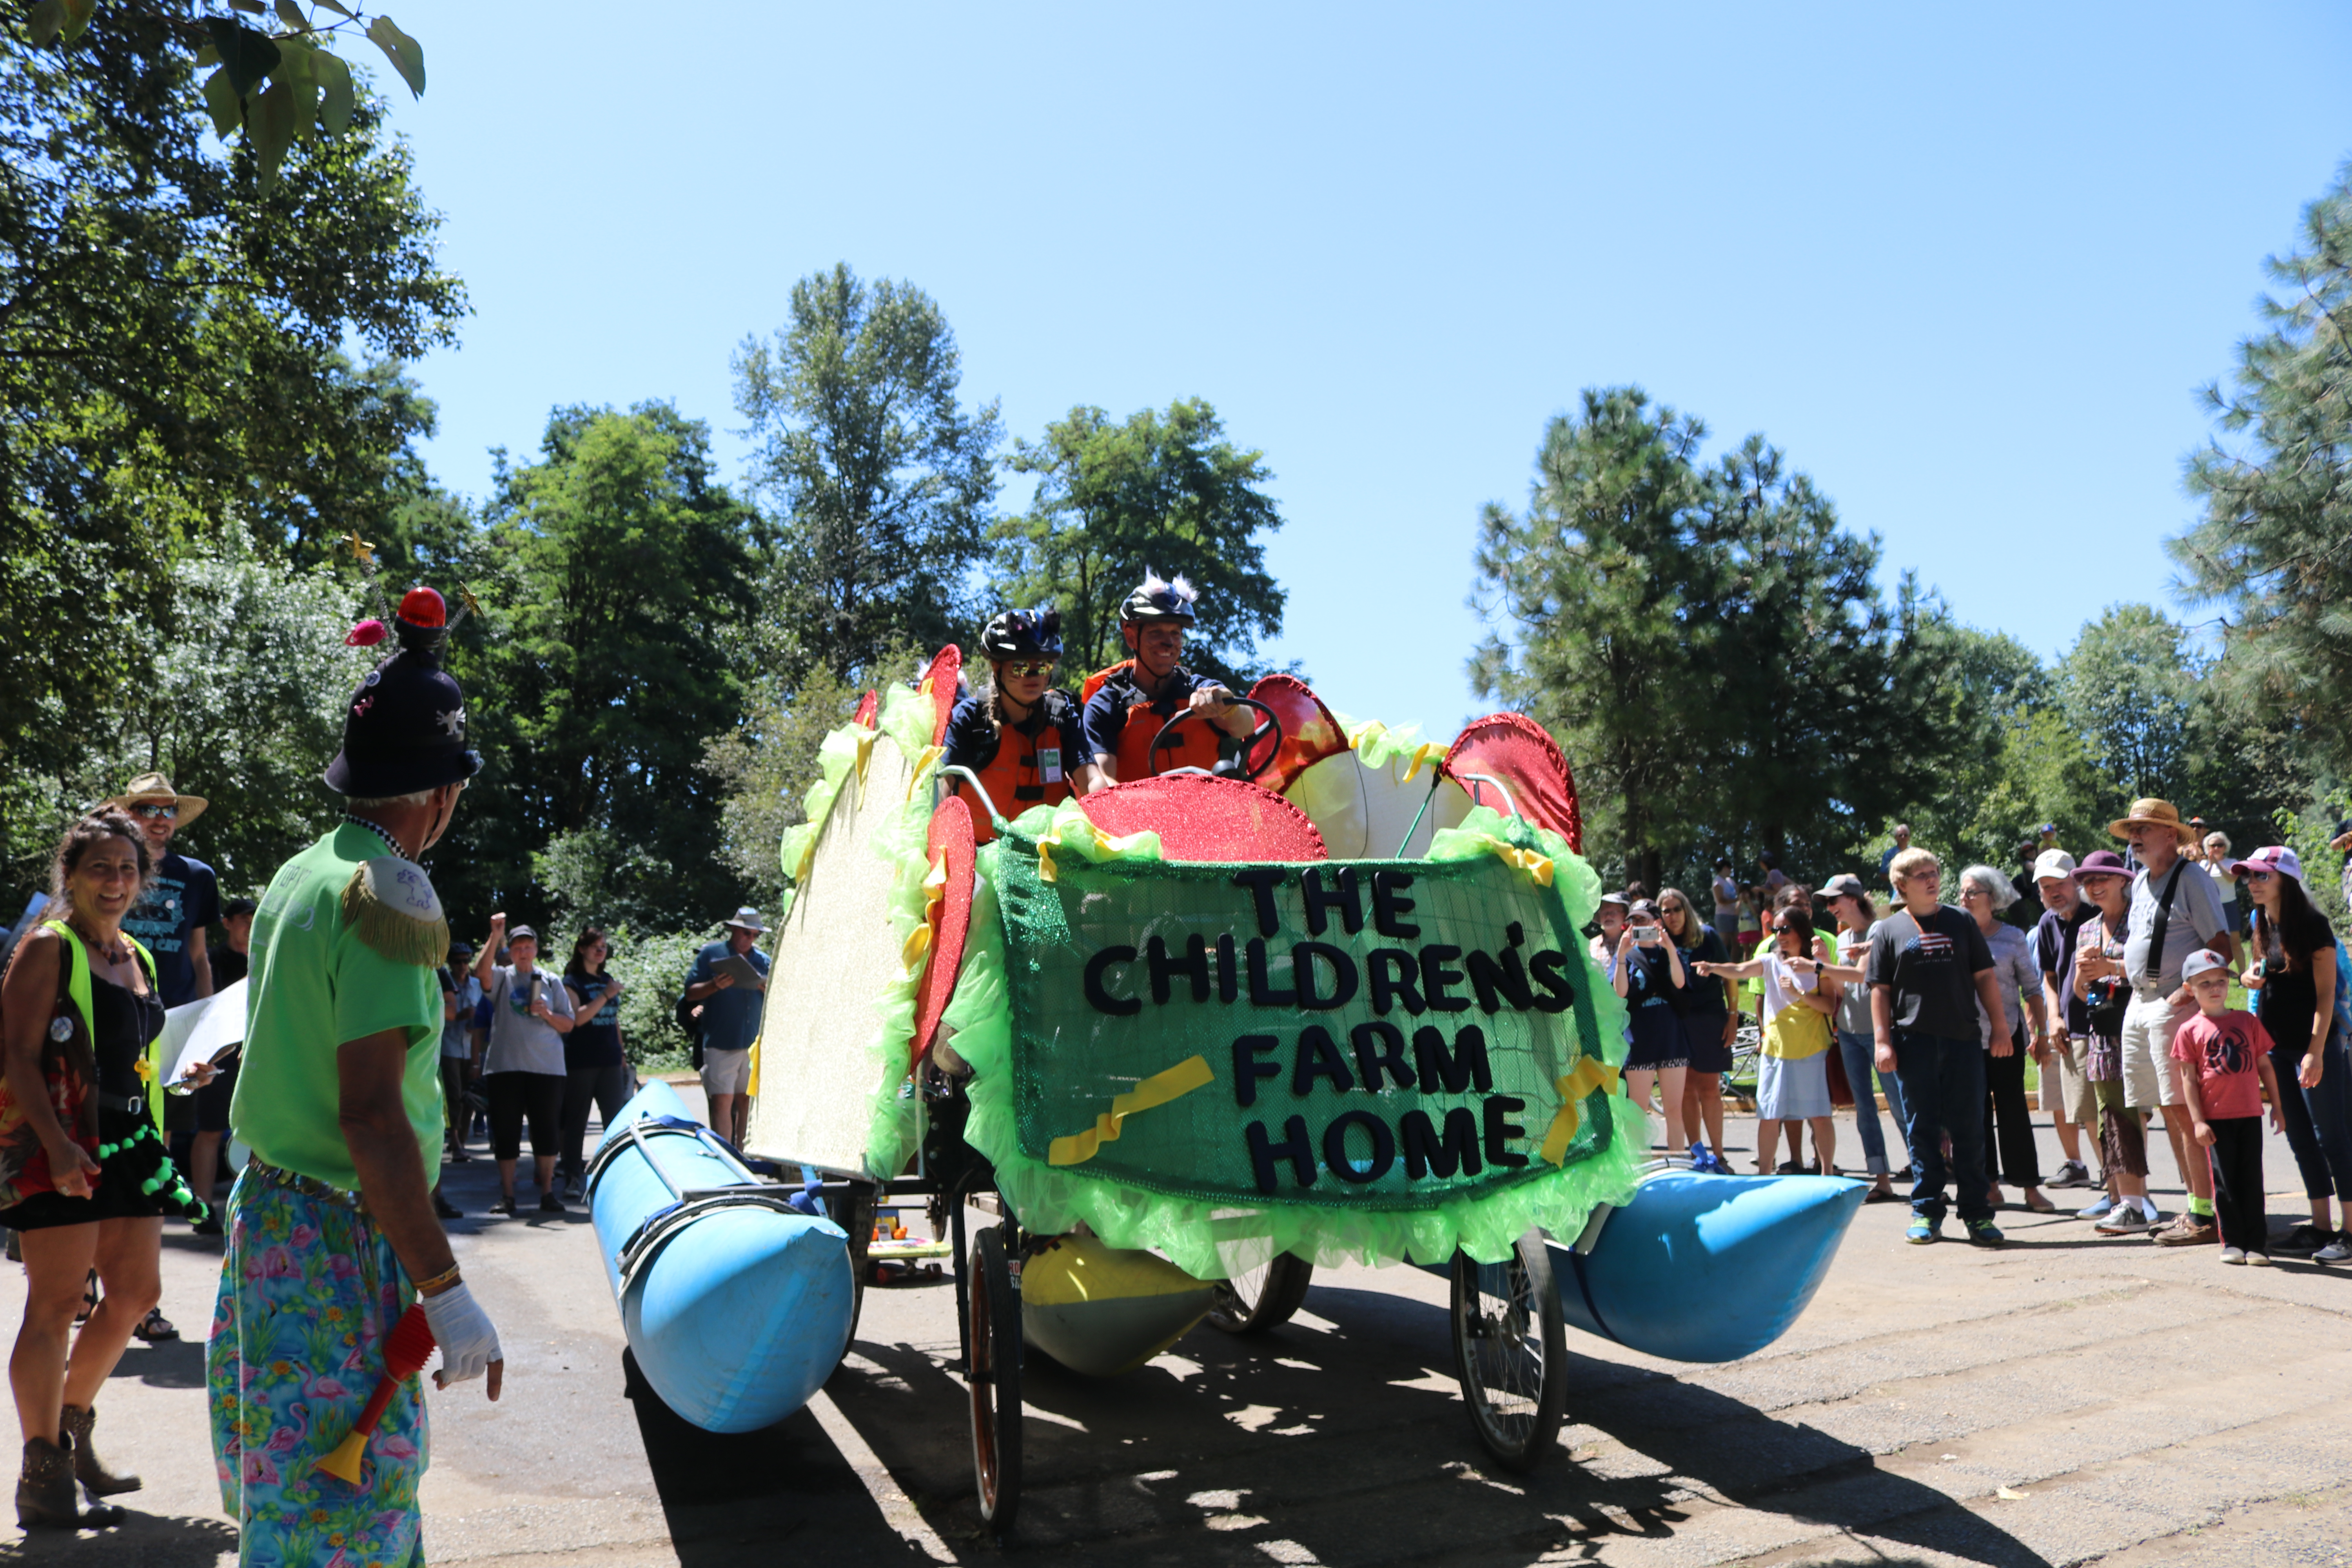
\includegraphics[height=.8\textheight]{media/IMG-2019-07-21-12160360.JPG}
	\end{center}
\end{frame}

\begin{frame}
	\begin{center}
		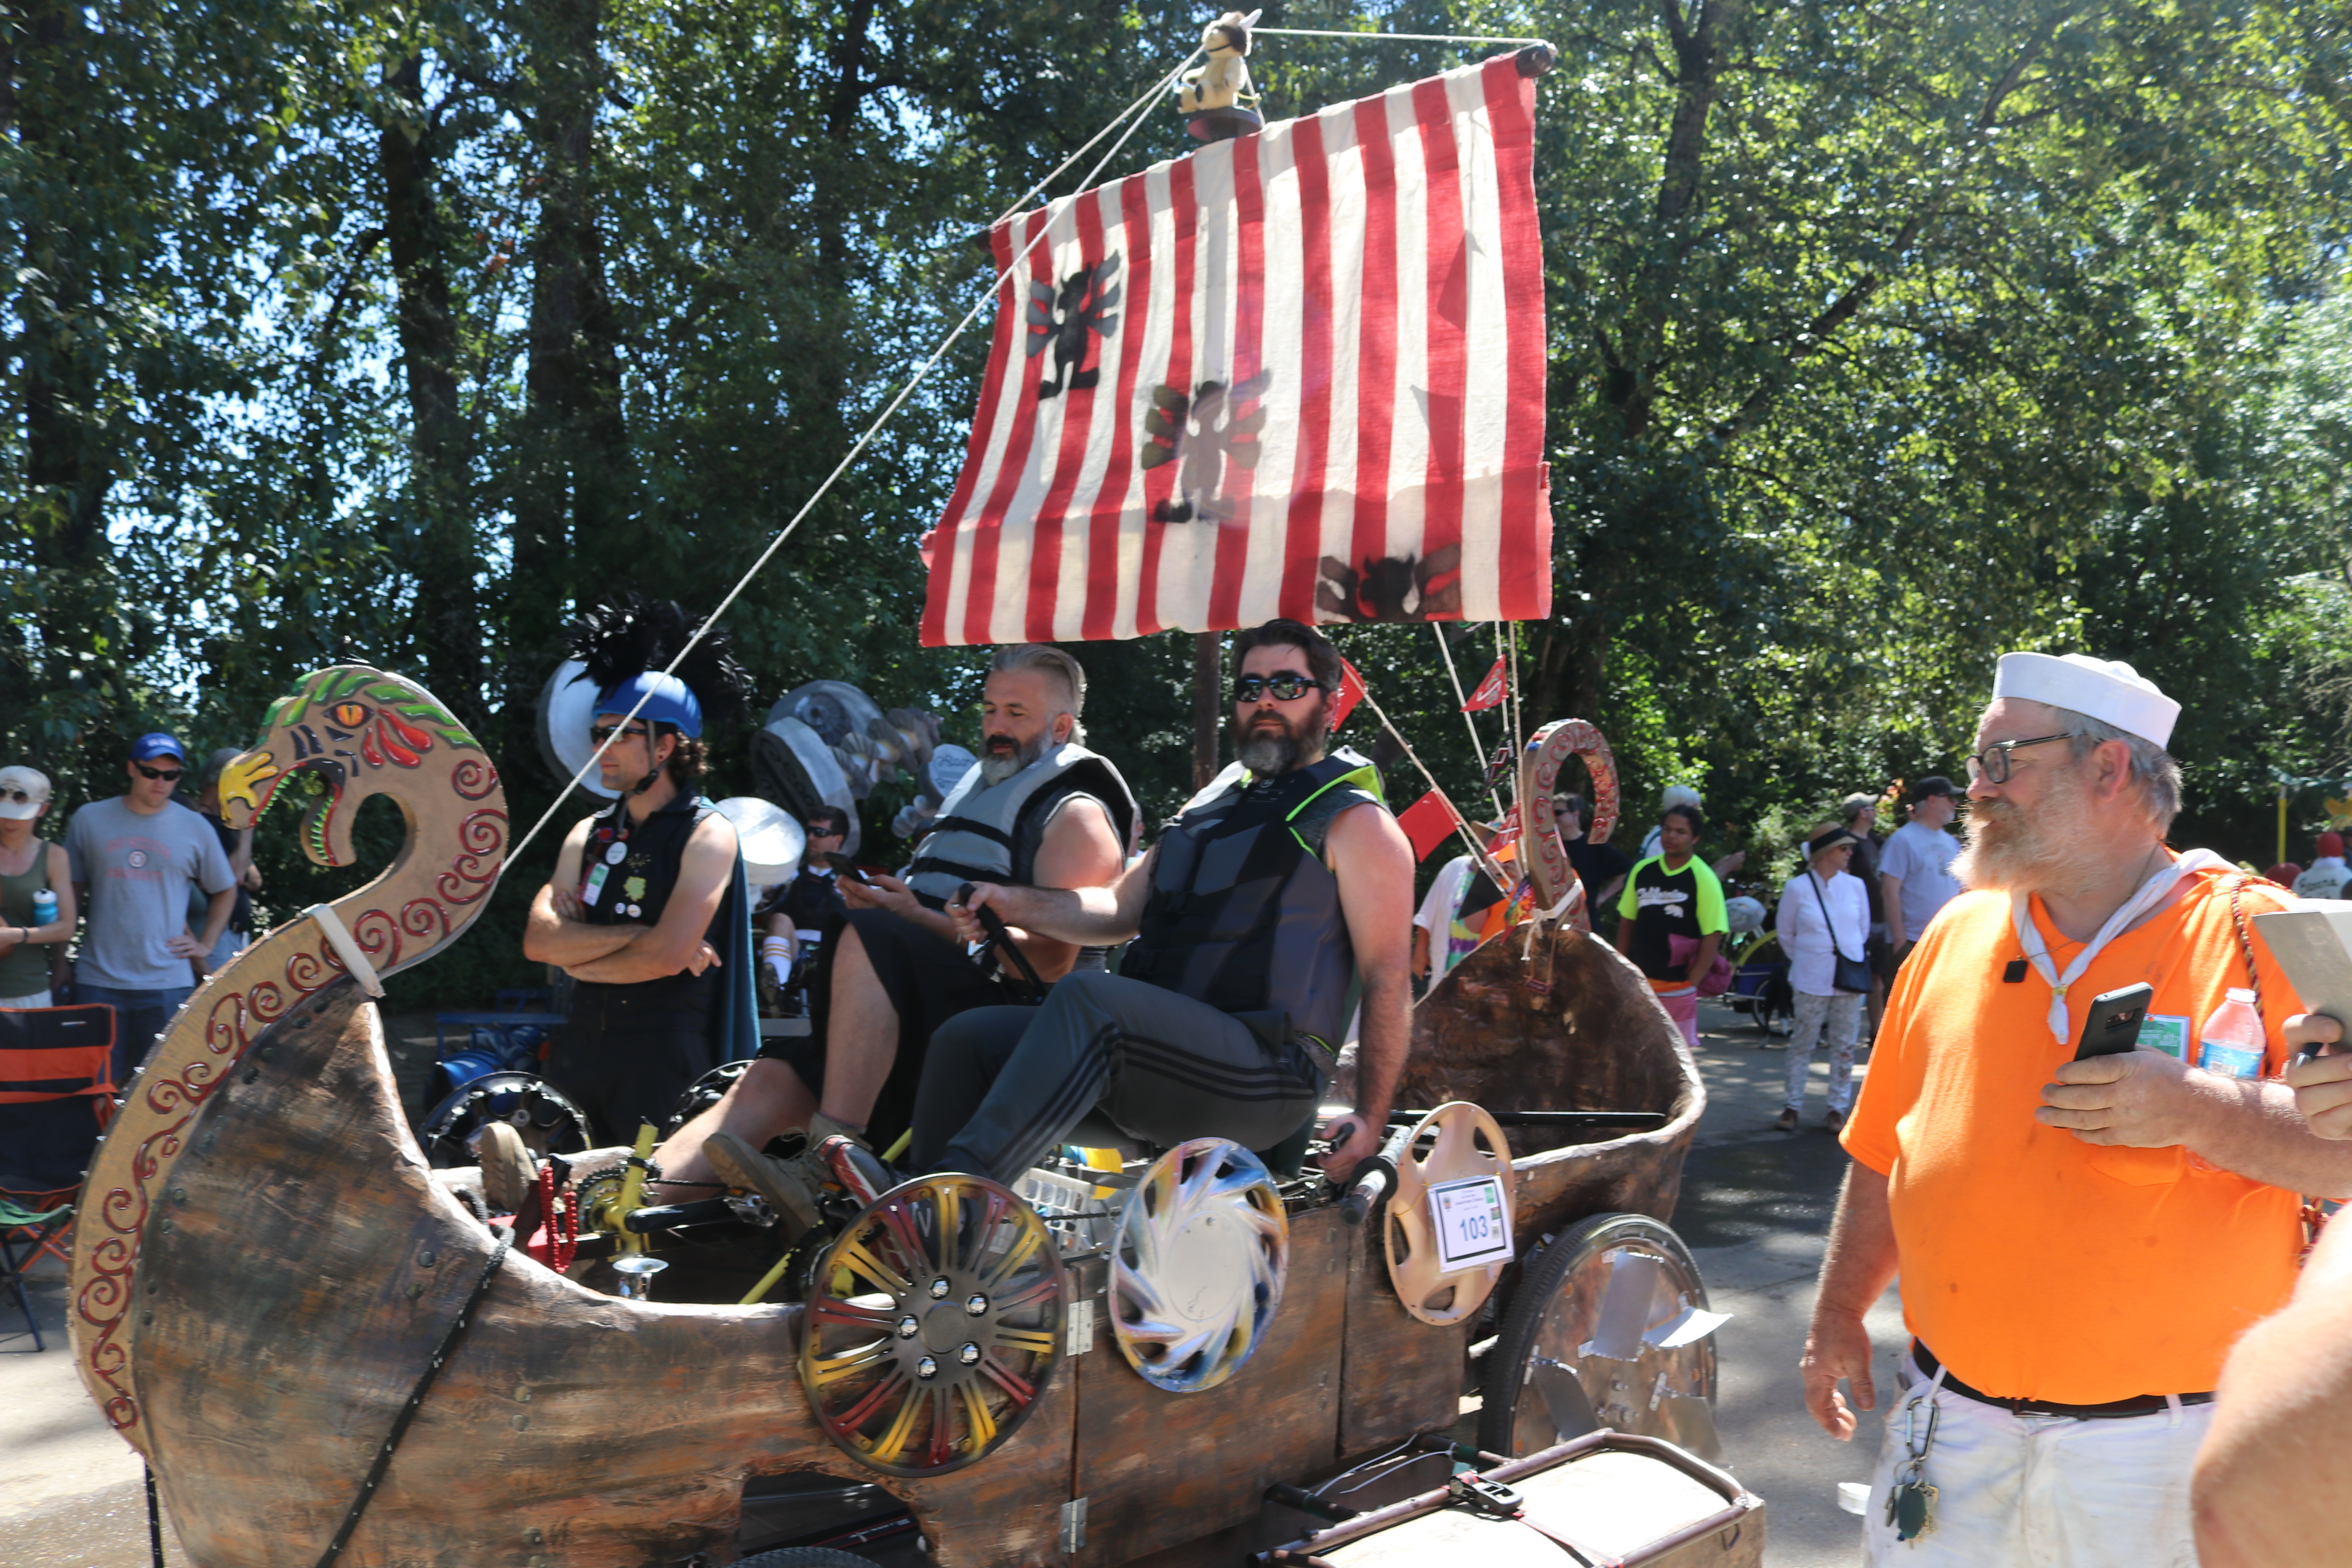
\includegraphics[height=.8\textheight]{media/IMG-2019-07-21-11502800.JPG}
	\end{center}
\end{frame}

\end{document}